\section{Methods}\label{methods}

In this section the underlying concepts and technologies are described. It starts with a brief description of XNAT and OpenStack. For further information about these systems and how they are integrated in the platform see~\cite{wu14}. The section continues with introducing the concept of workflows, the functionalities of WS-PGRADE/gUSE and the DCI-Bridge, which is an important part of gUSE. The last subsection describes a sample application, which has been used throughout the project.

\subsection{XNAT}\label{xnat}

TODO

\subsection{OpenStack}\label{openstack}

TODO

\subsection{Workflows}\label{workflows}

Applications consist of executable programs.
They usually take input, which can be in the form of command-line parameters or files and produce output files.
Some programs depend on the output of other programs, so that a mechanism is needed to ensure that all required inputs have been produced successfully before the program runs.
The workflow itself is a description or recipe how to link the executables together and are often stored in xml formats.
In terms of a workflow, every program is described as job, which can consist of one executable file or as in gUSE can be a zip file containing several files.
Every job has input and output ports, where each port has a number to identify it.
There can only be one file assigned to each port, which is then used to execute the program.
Every output port of one job can be linked to an input port of another program.
A system like gUSE that implements workflows ensures that the all necessary inputs are available before the job is started.
The produced data is then transported to the expected location where next job can see it.
When a job fails, it can resume this single job after the problem has been fixed.
There is no need to process all the successfully finished jobs again.
One of the most important feature of the ports is the support of naming conventions.
An input file assigned to a port is renamed, so that the program can find it in the storage.
The program also produces files that are named in a special way.
This name must be specified for the output port, so that the workflow system can keep track of the produced files.
Different jobs that have linked outputs and inputs can follow different naming conventions.

\subsection{WS-PGRADE/gUSE}\label{guse}

Grid and cloud User Support Environment (gUSE) is an opensource workflow management system developed at the Laboratory of Parallel and Distributed Systems in Hungaria.
WS-PGRADE is a collection of several gUSE Java Enterprise services that are combined to form a full featured e-science portal.
It provides a user-interface based on the opensource portal software Liferay.

The web portal is used to create and manage workflows. In order to create a new workflow three steps necessary. First a graph is created using a Java Applet named graph editor, which is provided on the portal. With the graph editor new jobs can be created and their ports can be connected (see section~\ref{workflows}). Figure~\ref{fig:grapheditor} shows a graph in the editor. The jobs are symbolized by yellow squares. Input ports are green, while output ports are gray. The arrows symbolize connections.
The graph is used to create a concrete workflow instance, which in the last step has to be configured.
The concrete workflows are shown in the user interface as can be seen in figure~\ref{fig:interfaceworkflows}.
During the configuration the executable programs and necessary command-line parameters are assigned to each job and input files are uploaded and assigned to the ports.
Also predefined middlewares can be selected, which define the platform to execute the workflows (see section~\ref{dci}).
The finalized workflow is then submitted to be executed.
The details button shows the status of the submitted workflows, wether they are running, finished or failed with an error.
Once a workflow is finished the resulting files, defined by the output ports can be downloaded as a .zip file.
Failed workflows can be resumed after the problem has been solved.


\begin{figure*}%[!b]
                \centering
                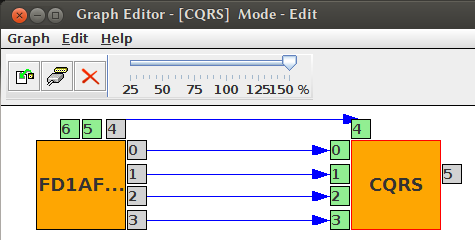
\includegraphics[width=1.0\columnwidth]{images/graph-editor.png}
                \caption{Graph editor of WS-PGRADE}
                \label{fig:grapheditor}
\end{figure*}

\begin{figure*}%[!b]
                \centering
                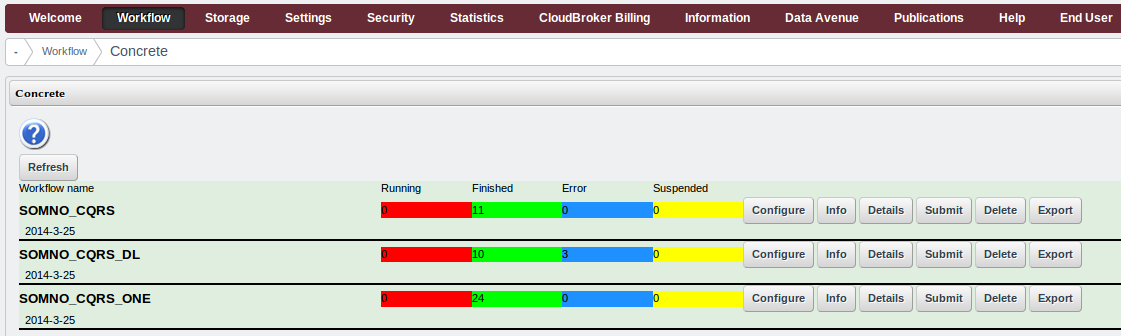
\includegraphics[width=2.0\columnwidth]{images/interface-workflows.png}
                \caption{List of concrete workflows in the web portal}
                \label{fig:interfaceworkflows}
\end{figure*}


\subsection{DCI-Bridge}\label{dci}

The DCI-Bridge is part of gUSE and connects the workflow system with different types of Distributed Computing Infrastructures (DCI).
These middlewares are for example grid or cloud infrastructures, where applications can be executed.
The DCI-Bridge is a generic interface receiving requests from the workflow system.
Different DCI plugins handle these request for different infrastructure types.
To connect a cloud infrastructure the DCI-Bridge provides a CloudBroker and a EC2 plugin.
Cloudbroker is an external service which is used to connect to a cloud.
As the SOMNO.Netz server architecture is encapsulated in a private network, which can not be reached from outside, this is not a suitable option.
Instead the EC2 plugin is being used, which connects to the cloud directly by talking to the EC2 interface of OpenStack (see section~\ref{openstack}), using the opensource command-line software euca-tools.

\subsection{Sample Applications}\label{applications}

TODO

\subsection{Workflow Repositories}\label{repositories}

TODO